\documentclass[tikz]{standalone}

\begin{document}

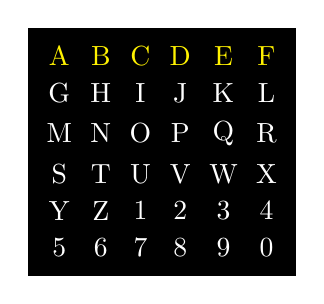
\begin{tikzpicture}
\def\xs{1} %shift in x direction
\def\ys{0.5} %shift in y direction
\def\nm{1} % number of 2d matrices in the 3d matrix
\def\x{1}
\makeatletter
\usetikzlibrary{calc}
\newcommand*\circled[1]{\tikz[baseline=(char.base)]{
    \node[shape=circle, draw, inner sep=1pt, 
        minimum height={\f@size*1.6},] (char) {\vphantom{WAH1g}#1};}}
\makeatother
\matrix [draw, % for the rectangle border
         fill=black, % so that it is not transparent
         ampersand replacement=\&] %see explanation
(mm\x)%give the matrix a name
at(-\x * \xs, -\x * \ys) %shift the matrix
{   
    \color{yellow} \node {A}; \& \color{yellow} \node {B}; \& \color{yellow} \node {C}; \& \color{yellow} \node {D}; \& \color{yellow} \node {E}; \& \color{yellow} \node {F};\\
    \color{white} \node {G}; \& \color{white} \node {H}; \& \color{white} \node {I}; \& \color{white} \node {J}; \& \color{white} \node {K}; \& \color{white}   \node {L};\\
    \color{white} \node {M}; \& \color{white} \node {N}; \& \color{white} \node {O}; \& \color{white} \node {P}; \& \color{white} \node {Q}; \& \color{white} \node {R};\\
\color{white} \node {S}; \& \color{white} \node {T}; \& \color{white} \node{U}; \& \color{white} \node {V}; \& \color{white} \node {W}; \& \color{white} \node {X};\\
\color{white} \node {Y}; \& \color{white} \node {Z}; \& \color{white} \node {1}; \& \color{white} \node {2}; \& \color{white} \node {3}; \& \color{white} \node {4};\\
\color{white} \node {5}; \& \color{white} \node {6}; \& \color{white} \node {7}; \& \color{white} \node {8}; \& \color{white} \node {9}; \& \color{white} \node {0};\\
};
%lalala
\end{tikzpicture}
\end{document}
